\documentclass[FIPLY_base.tex]{subfiles}

%\author{Daniel Bersenkowitsch}
	
\begin{document}
	\ \\
	\subsection{Design}
	Die Hintergrundgfarbe aller Activities ist ein starkes Grau, die Entscheidung viel schlussendlich auf die Farbe mit dem Farbcode \#363534. Die dazu kontraste Signalfarbe ist ein eindeutiges Orange, \#ff8400. Der Kontrast dieser zwei Farben ist ein guter Blickfang und angenehm für das Augen. Als Kontur wird ein einfaches Schwarz (\#000000) herangezogen. Durch diese drei Hauptfarben wird dem Benutzer ein visuell-angenehmes Farbenspektrum geboten, wodurch eine klare Übersicht über alle Elemente entsteht.
	\begin{itemize}
	 	\item Hauptfarbe/Kontrastfarbe: \#ff8400 (Orange)
	 	\item Hintergrundfarbe: \#ff8400 (Grau)
	 	\item Konturfarbe: \#000000 (Schwarz)
	\end{itemize}
	Alle weitere Farben entsprechen einem verwandten Farbton, die jedoch nicht erwähnenswert sind.
	
	\subsubsection{FIPLY-Logo} 
	Am Anfang war das Ziel des FIPLY-Logos, dem Benutzer bei der Ansicht des Bildes intuitiv zu vermitteln, dass es sich um eine Fitness Applikation handelt. Dies geschieht einfach mit verschiedenen fitnesstypischen Formen, wie zum Beispiel eine Hantel, ein laufender Mensch, ein Muskulöser Arm oder auch nur einen Turnschuh. Da die Applikation das Generieren eines Fitnessplans anbietet, wurde entschieden, eine Art Kalender-Logo daraus zu machen. 
	\begin{figure}[H]
		\begin{subfigure}[b]{1\textwidth}
			\centering
			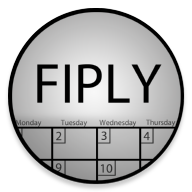
\includegraphics[scale=1]{img/icons/Version1}
			\centering
			\caption{Version 1 des FIPLY Logos}
		\end{subfigure}
	\end{figure}
	\ \\
	In der ersten Version des FIPLY Logos (Grafik a dieses Abschnitts) umfasst nur einen Schwarz-Weiß Farbstil mit einem zentrierten \grqq{}FIPLY\grqq{} Schriftzug. Darunter findet sich das Bild eines typischen Kalenders, dass die Involvierung eines Plans suggestieren soll. Da es in den Augen der Projektmitglieder aber zu wenig Wiedererkennungswert aufweißt, wurde entschieden, ein neues Logo zu entwerfen. 
	\ \\
	Ziel ist es diesmal, ein Logo zu erstellen, das großen Wiedererkennungswert besitzt und sich gleichzeitig von anderen Logos auf eine individuelle Art und Weise heraussticht. Dabei kann die Suggestierung an den Fitnessbreich vernachlässigt werden. Ein möglichst einfach gehaltenes Logo mit ebenso einfachen Farben, ohne Farbverlauf. Dabei wird auf das Standardfarbschema des FIPLY Projekts zurückgegriffen:
	\begin{figure}[H]
		\begin{subfigure}[b]{1\textwidth}
			\centering
			
\includegraphics[scale=0.75]{img/icons/Version2}
			\centering
			\caption{Version 2 des FIPLY Logos}
		\end{subfigure}
	\end{figure}
	\subsubsection{Kontrollelemente}
	Als Hintergrundfarbe der Kontrollelemente wird die Hauptfarbe angwendet. Bei normalen Textelementen kommt die Hauptfarbe zum Einsatz, bei jeden anderen texthaltigen Elementen wird etwa die Konturfarbe oder Hintergrundfarbe eingesetzt. Dies wird mittels Icons umgesetzt. Das jeweilig erstellte Icon wird als Hintergrundbild eines Kontrollelements programmiert. Folgende wichtige Icons wurden für Kontrollelemente eingesetzt, das jeweilige Icon wird eingesetzt für *:
	
	\begin{figure}[H]
		\begin{subfigure}[b]{0.2\textwidth}
			
\includegraphics[scale=0.5]{img/icons/play}
			\caption{* den play-Knop des Musikplayers}
		\end{subfigure}
		\hfil
		\begin{subfigure}[b]{0.2\textwidth}
			
\includegraphics[scale=0.5]{img/icons/pause}
			\caption{* den pause-Knopfdes Musikplayers}
		\end{subfigure}
		\hfil
		\begin{subfigure}[b]{0.2\textwidth}
			
\includegraphics[scale=0.5]{img/icons/last}
			\caption{* den voriger Song-Knopf des Musikplayers}
		\end{subfigure}
		\hfil
		\begin{subfigure}[b]{0.2\textwidth}
			
\includegraphics[scale=0.5]{img/icons/next}
			\caption{* den nächster Song-Knopf des Musikplayers}
		\end{subfigure}
		\hfil
		\begin{subfigure}[b]{0.2\textwidth}
			
\includegraphics[scale=0.5]{img/icons/successsmall}
			\caption{* eine Erfolgsmeldung}
		\end{subfigure}
		\hfil
		\begin{subfigure}[b]{0.2\textwidth}
			
\includegraphics[scale=0.5]{img/icons/questionsmall}
			\caption{* eine Abfrage}
		\end{subfigure}
		\hfil
		\begin{subfigure}[b]{0.2\textwidth}
			
\includegraphics[scale=0.5]{img/icons/alertsmall}
			\caption{* eine Fehlermeldung}
		\end{subfigure}
		\hfil
		\begin{subfigure}[b]{0.2\textwidth}
			
\includegraphics[scale=0.5]{img/icons/stop}
			\caption{* den stop-Knopf des Musikplayers}
		\end{subfigure}
		\hfil
		\begin{subfigure}[b]{0.2\textwidth}
			
\includegraphics[scale=0.5]{img/icons/informationsmall}
			\caption{* einen Informations-Knopf}
		\end{subfigure}
		\hfil
		\begin{subfigure}[b]{0.2\textwidth}
			
\includegraphics[scale=0.5]{img/icons/star_emptysmall}
			\caption{* einen leeren Bewertungstern}
		\end{subfigure}
		\hfil
		\begin{subfigure}[b]{0.2\textwidth}
			
\includegraphics[scale=0.5]{img/icons/listviewunpressed}
			\caption{* eine (spezielle) Listenbearbeitung, ungedrückt}
		\end{subfigure}
		\hfil
		\begin{subfigure}[b]{0.2\textwidth}
			
\includegraphics[scale=0.5]{img/icons/stopwatch}
			\caption{* die Stoppuhr}
		\end{subfigure}
		\hfil
		\begin{subfigure}[b]{0.2\textwidth}
			
\includegraphics[scale=0.5]{img/icons/exportcsvsmall}
			\caption{* den exportieren-Knopf}
		\end{subfigure}
		\hfil
		\begin{subfigure}[b]{0.2\textwidth}
			
\includegraphics[scale=0.5]{img/icons/starsmall}
			\caption{* einen vollen Bewertungstern}
		\end{subfigure}
		\hfil
		\begin{subfigure}[b]{0.2\textwidth}
			
\includegraphics[scale=0.5]{img/icons/listviewpressed}
			\caption{* eine (spezielle) Listenbearbeitung, gedrückt}
		\end{subfigure}
		\hfil
		\begin{subfigure}[b]{0.2\textwidth}
			
\includegraphics[scale=0.5]{img/icons/countdown}
			\caption{* eine countdown Uhr}
		\end{subfigure}
		\hfil
		\begin{subfigure}[b]{0.2\textwidth}
			
\includegraphics[scale=0.5]{img/icons/minusgreysmall}
			\caption{* das löschen eines Elements, ungedrückt}
		\end{subfigure}
		\hfil
		\begin{subfigure}[b]{0.2\textwidth}
			
\includegraphics[scale=0.5]{img/icons/minusorangesmall}
			\caption{* das löschen eines Elements, gedrückt}
		\end{subfigure}
		\hfil
		\begin{subfigure}[b]{0.2\textwidth}
			
\includegraphics[scale=0.5]{img/icons/plusgreysmall}
			\caption{* das hinzufügen eines Elements, ungedrückt}
		\end{subfigure}
		\hfil
		\begin{subfigure}[b]{0.2\textwidth}
			
\includegraphics[scale=0.5]{img/icons/plusorangesmall}
			\caption{* das löschen eines Elements, gedrückt}
		\end{subfigure}
		\hfil
		\begin{subfigure}[b]{0.2\textwidth}
			
\includegraphics[scale=0.5]{img/icons/simplelistviewpressed}
			\caption{* eine (normale) Listenbearbeitung, gedrückt}
		\end{subfigure}
		\hfil
		\begin{subfigure}[b]{0.2\textwidth}
			
\includegraphics[scale=0.5]{img/icons/simplelistviewunpressed}
			\caption{* eine (normale) Listenbearbeitung, ungedrückt}
		\end{subfigure}
		\hfil
		\begin{subfigure}[b]{0.2\textwidth}
			
\includegraphics[scale=0.8]{img/icons/toggleoffsmall}
			\caption{* einen Toggle-Knopf, ein}
		\end{subfigure}
		\hfil
		\begin{subfigure}[b]{0.2\textwidth}
			
\includegraphics[scale=0.8]{img/icons/toggleonsmall}
			\caption{* einen Toggle-Knopf, aus}
		\end{subfigure}
		\hfil

	\end{figure}
	
	
\end{document}